\section{Mottos}\label{sec:mottos}

\begin{wrapfigure}{R}{0.3\textwidth}
    \centering
    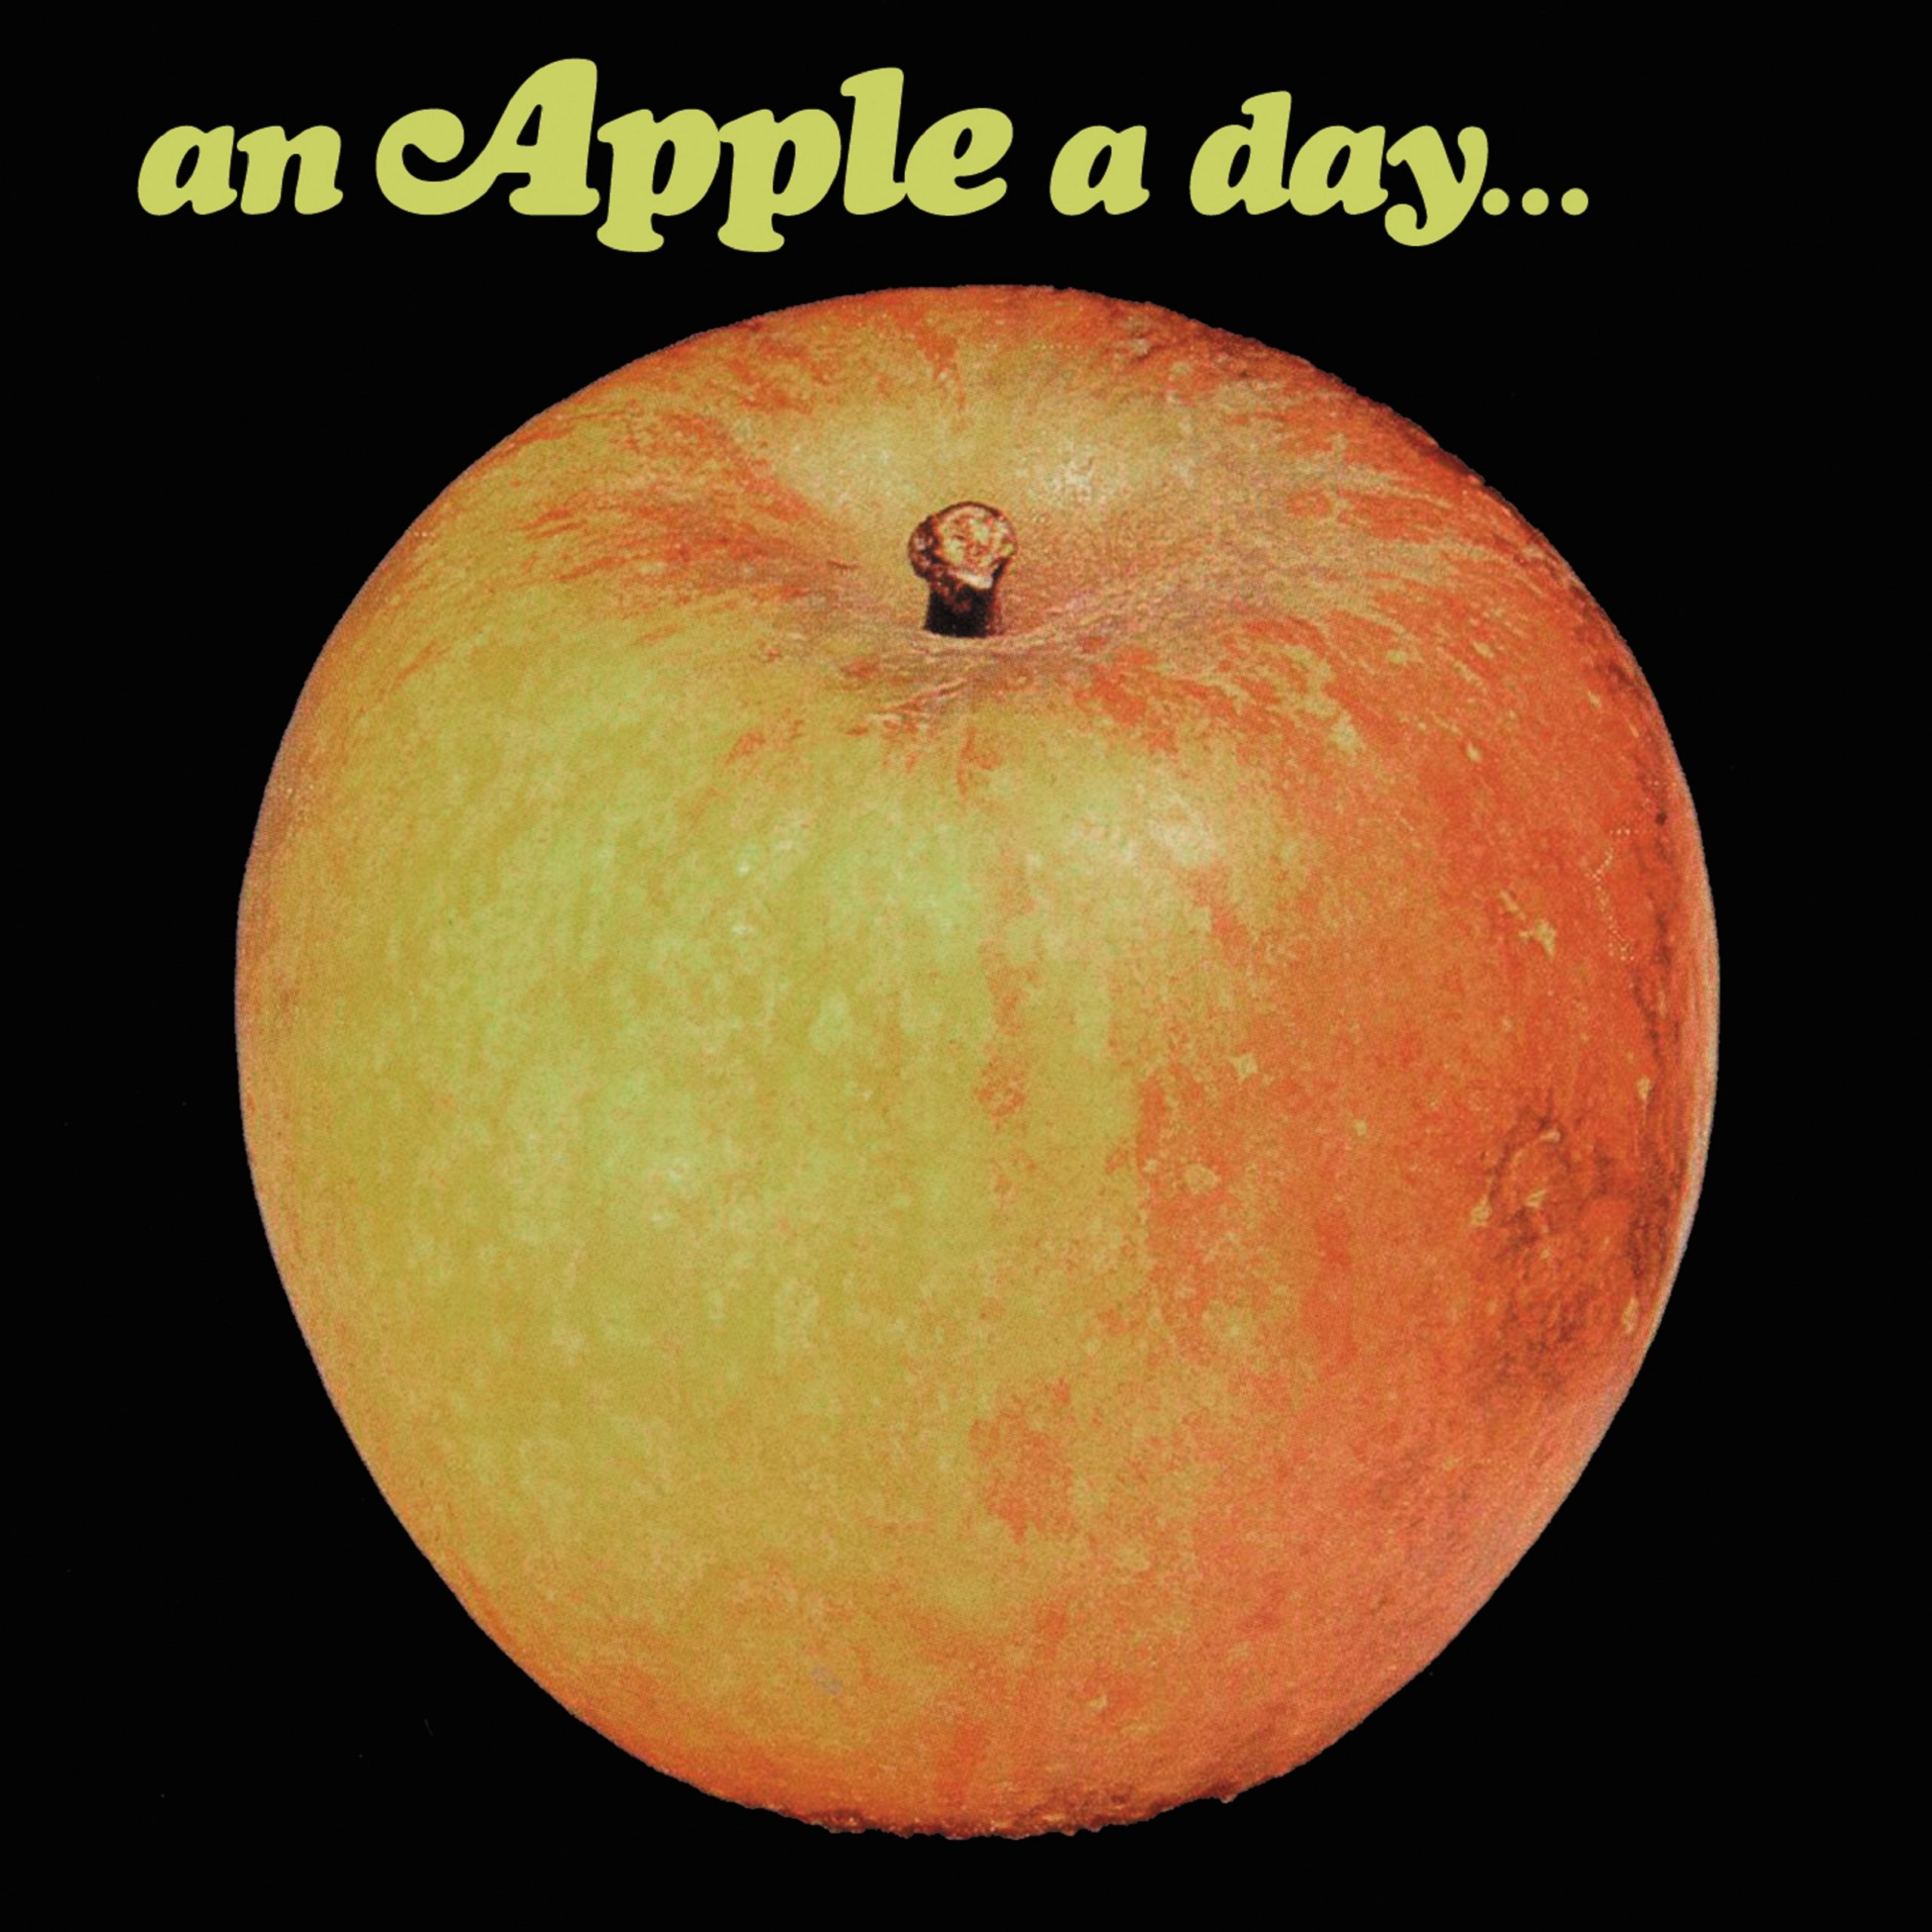
\includegraphics[width=0.25\textwidth]{images/mottos}
\end{wrapfigure}

You could also call them (universal) guidelines, which are semantically more specific than principles, yet not as specific as concrete techniques.
They help us improve our technique, implement the principles, and embody a CI quality.
They are kept short, so we can remember them quickly, and can act as part of our vocabulary (but then just longer):
Once we mention it to someone who is also familiar with that saying, we immediately have a common understanding within a very short period of time.

\subsection{Examples}\label{subsec:examples}

\begin{itemize}
    \item \textit{Tension masks sensation.} Imagine your muscles are tensing up so much, they squeeze the nerves which then can't transmit any information anymore.
    The more relaxed we are, the more sensitive our skin is to touch and pressure/weight.
    \item \textit{Keep on breathing.} When getting tensed up, physically and emotionally, we humans tend to hold our breath, which is counterproductive to stay sharp, focused and relaxed.
    Instead, we continuously try to remind ourselves to breath, and especially emphasize a deep out-breath.
    \item \textit{We try not to fall in love with our partner, we fall in love with the dance.} Try to depersonalize your dance partner, seeing him as a mere physical object and by that explore the physical realm instead of the psychological, interpersonal realm.
    It's also not a personal dance, it's a physicality; the experience is because of the practice, not because of your partner necessarily; don't attach that to a specific person.
    Even when you had an amazing dance with someone, once the dance is over, I'm going to say ``thank you, and bye bye''.
    It is nevertheless possible of course to talk to that person later on, but not lingering and dance the entire class or jam with that single person.
    \item \textit{Keep eyes open and ``wide''.} Sometimes people tend to close them, or focus them on the partner.
    Instead, we want to keep an open gaze, perceiving everything around us, staying in connection with all the people in the room and the room itself.
    Once we start to gaze at the floor, this is usually an indication of a hyper-focus which potentially closes our perception.
    \item \textit{Dance at the edge of your level of attention, and don't cross the level of your partner's attention.} Try to expand what you are able to do in regard to movement, attention, speed, techniques, and pathways.
    And very important, listen to what your partner is able as well.
\end{itemize}

\subsection{Mistakes}\label{subsec:mistakes}

As in general with any improvised art, mistakes are only seen as such as soon as we declare them as being mistakes.

Imagine two improvisation actors on stage.
One says mouse, the other house.
And then again, the same thing: house - mouse.
They actually intended to go on with different rhyming words, but for whatever reason (too nervous?) they are stuck and can't come up with something new, and because they are able to fake it as a deliberate decision (not admitting it being a mistake, something which was not their initial desired goal; when things don't go according to a fixed plan), people in the audience might be amazed by the ``post-modern acting skills'' and interpret something into it.

Once you are able to let go of any plan, and be truly in the present moment with whatever is happening; once you are able to fully comprehend that whenever there is another person involved, any desire for control is futile \ldots then you will be able to surrender and use any happening as a source of inspiration.
Ultimately being able ``to surprise yourself'', and be fascinated what happened to you.
